\documentclass[11pt]{article}
\usepackage[top=2cm,left=2cm,right=2cm,bottom=2cm]{geometry}
\usepackage[doublespacing]{setspace}
\usepackage{graphicx}
\usepackage{xcolor}
\usepackage{subfigure}
\usepackage[hidelinks]{hyperref}
\usepackage{amsmath}
\usepackage{amssymb}
\usepackage{lscape}
\usepackage{booktabs}
\usepackage{listings}
\usepackage{pythonhighlight}
\usepackage{tcolorbox}
\usepackage[localise]{xepersian}
\settextfont{XB Niloofar}

\definecolor{codegreen}{rgb}{0,0.6,0}
\definecolor{codegray}{rgb}{0.5,0.5,0.5}
\definecolor{codepurple}{rgb}{0.58,0,0.82}
\definecolor{backcolour}{rgb}{0.95,0.95,0.92}

\lstdefinestyle{mystyle}{
	backgroundcolor=\color{backcolour},   
	commentstyle=\color{codegreen},
	keywordstyle=\color{magenta},
	numberstyle=\tiny\color{codegray},
	stringstyle=\color{codepurple},
	basicstyle=\ttfamily\footnotesize,
	breakatwhitespace=false,         
	breaklines=true,                 
	captionpos=b,                    
	keepspaces=true,                 
	numbers=left,                    
	numbersep=5pt,                  
	showspaces=false,                
	showstringspaces=false,
	showtabs=false,                  
	tabsize=2
}
\lstset{style=mystyle}

\begin{document}
	\شروع{وسط‌چین}
	به نام خدا\\
	\vspace{1cm}
	\begin{figure}[h]
		\begin{center}
			\includegraphics[width=0.3\linewidth]{"D:/Logo/UT"}
		\end{center}
	\end{figure}
	{\درشت‌درشت دانشکده مهندسی مکانیک}\\
	\vspace{1cm}
	{\بزرگ \سیاه{نام درس: هوش مصنوعی}}\\
	
	\vspace{0.5cm}
	{\درشت‌درشت تمرین ۴(شبکه بازگشتی)}
	\vspace{1.5cm}
	
	\vspace{1.5cm}
	{\درشت‌درشت {\سیاه استاد درس:} دکتر شریعت‌پناهی}\\
	\vspace{2cm}
	{\درشت‌درشت {\سیاه دانشجو:}}\\
	{\درشت مهدی نوذری\\
	810601139}\\
	\vspace{3cm}
	بهار ۱۴۰۳\\
	\پایان{وسط‌چین}
	\pagebreak
		تمامی فایل‌ها در \lr{Github} موجود هستند:
	\href{https://github.com/Morphit/UT_AI_1403}{\lr{https://github.com/Morphit/UT\_AI\_1403}}
	
	\vspace{1cm}
	در این تمرین، هدف استفاده از تعدادی فایل صوتی شامل جملاتی به زبان آلمانی برای تربیت یک شبکه است که بتواند احساسات این جملات را تشخیص دهد. ابتدا داده‌ها باید گردآوری شده و در صورت نیاز داده‌افزایی صورت بگیرد،‌ سپس با پیش‌پردازش داده‌ها ویژگی‌های سیگنال‌ها در طول زمان استخراج می‌شوند.
	%در مرحله بعد با استفاده از این ویژگی‌ها شبکه‌هایی آموزش داده می‌شوند و عملکردشان مورد بررسی قرار می‌گیرد.
	\section{گرداوری داده‌ها}
	در این بخش باید داده‌ها را گردآوری کرده و \lr{Data frame} را تشکیل داد. چنانچه نام فایل‌ها را بررسی کنیم می‌توان دید که حرف ششم هر نام، برچسب آن را مشخص می‌کند و باید از آن برای برچسب‌زنی داده‌ها استفاده کرد. به این منظور در یک حلقه برای تمامی فایل‌ها ابتدا برچسب آن را پیدا کرده و داده‌های آن را به شکل یک سری زمانی استخراج می‌کنیم. با استفاده از این سری زمانی و دستور‌های 
	\verb|pitch_shift|
	و
	\verb|time_stretch|
	۶ داده جدید تولید می‌شود که به ترتیب تن صدا و سرعت متفاوتی دارند اما برچسب یکسانی با گفتار اولیه دارند. می‌توان یک نمونه‌ از هر تغییر را در
	\autoref{fig:shift}
	و
	\autoref{fig:stretch}
	مشاهده کرد.
	\begin{figure}[!h]
		\centerline{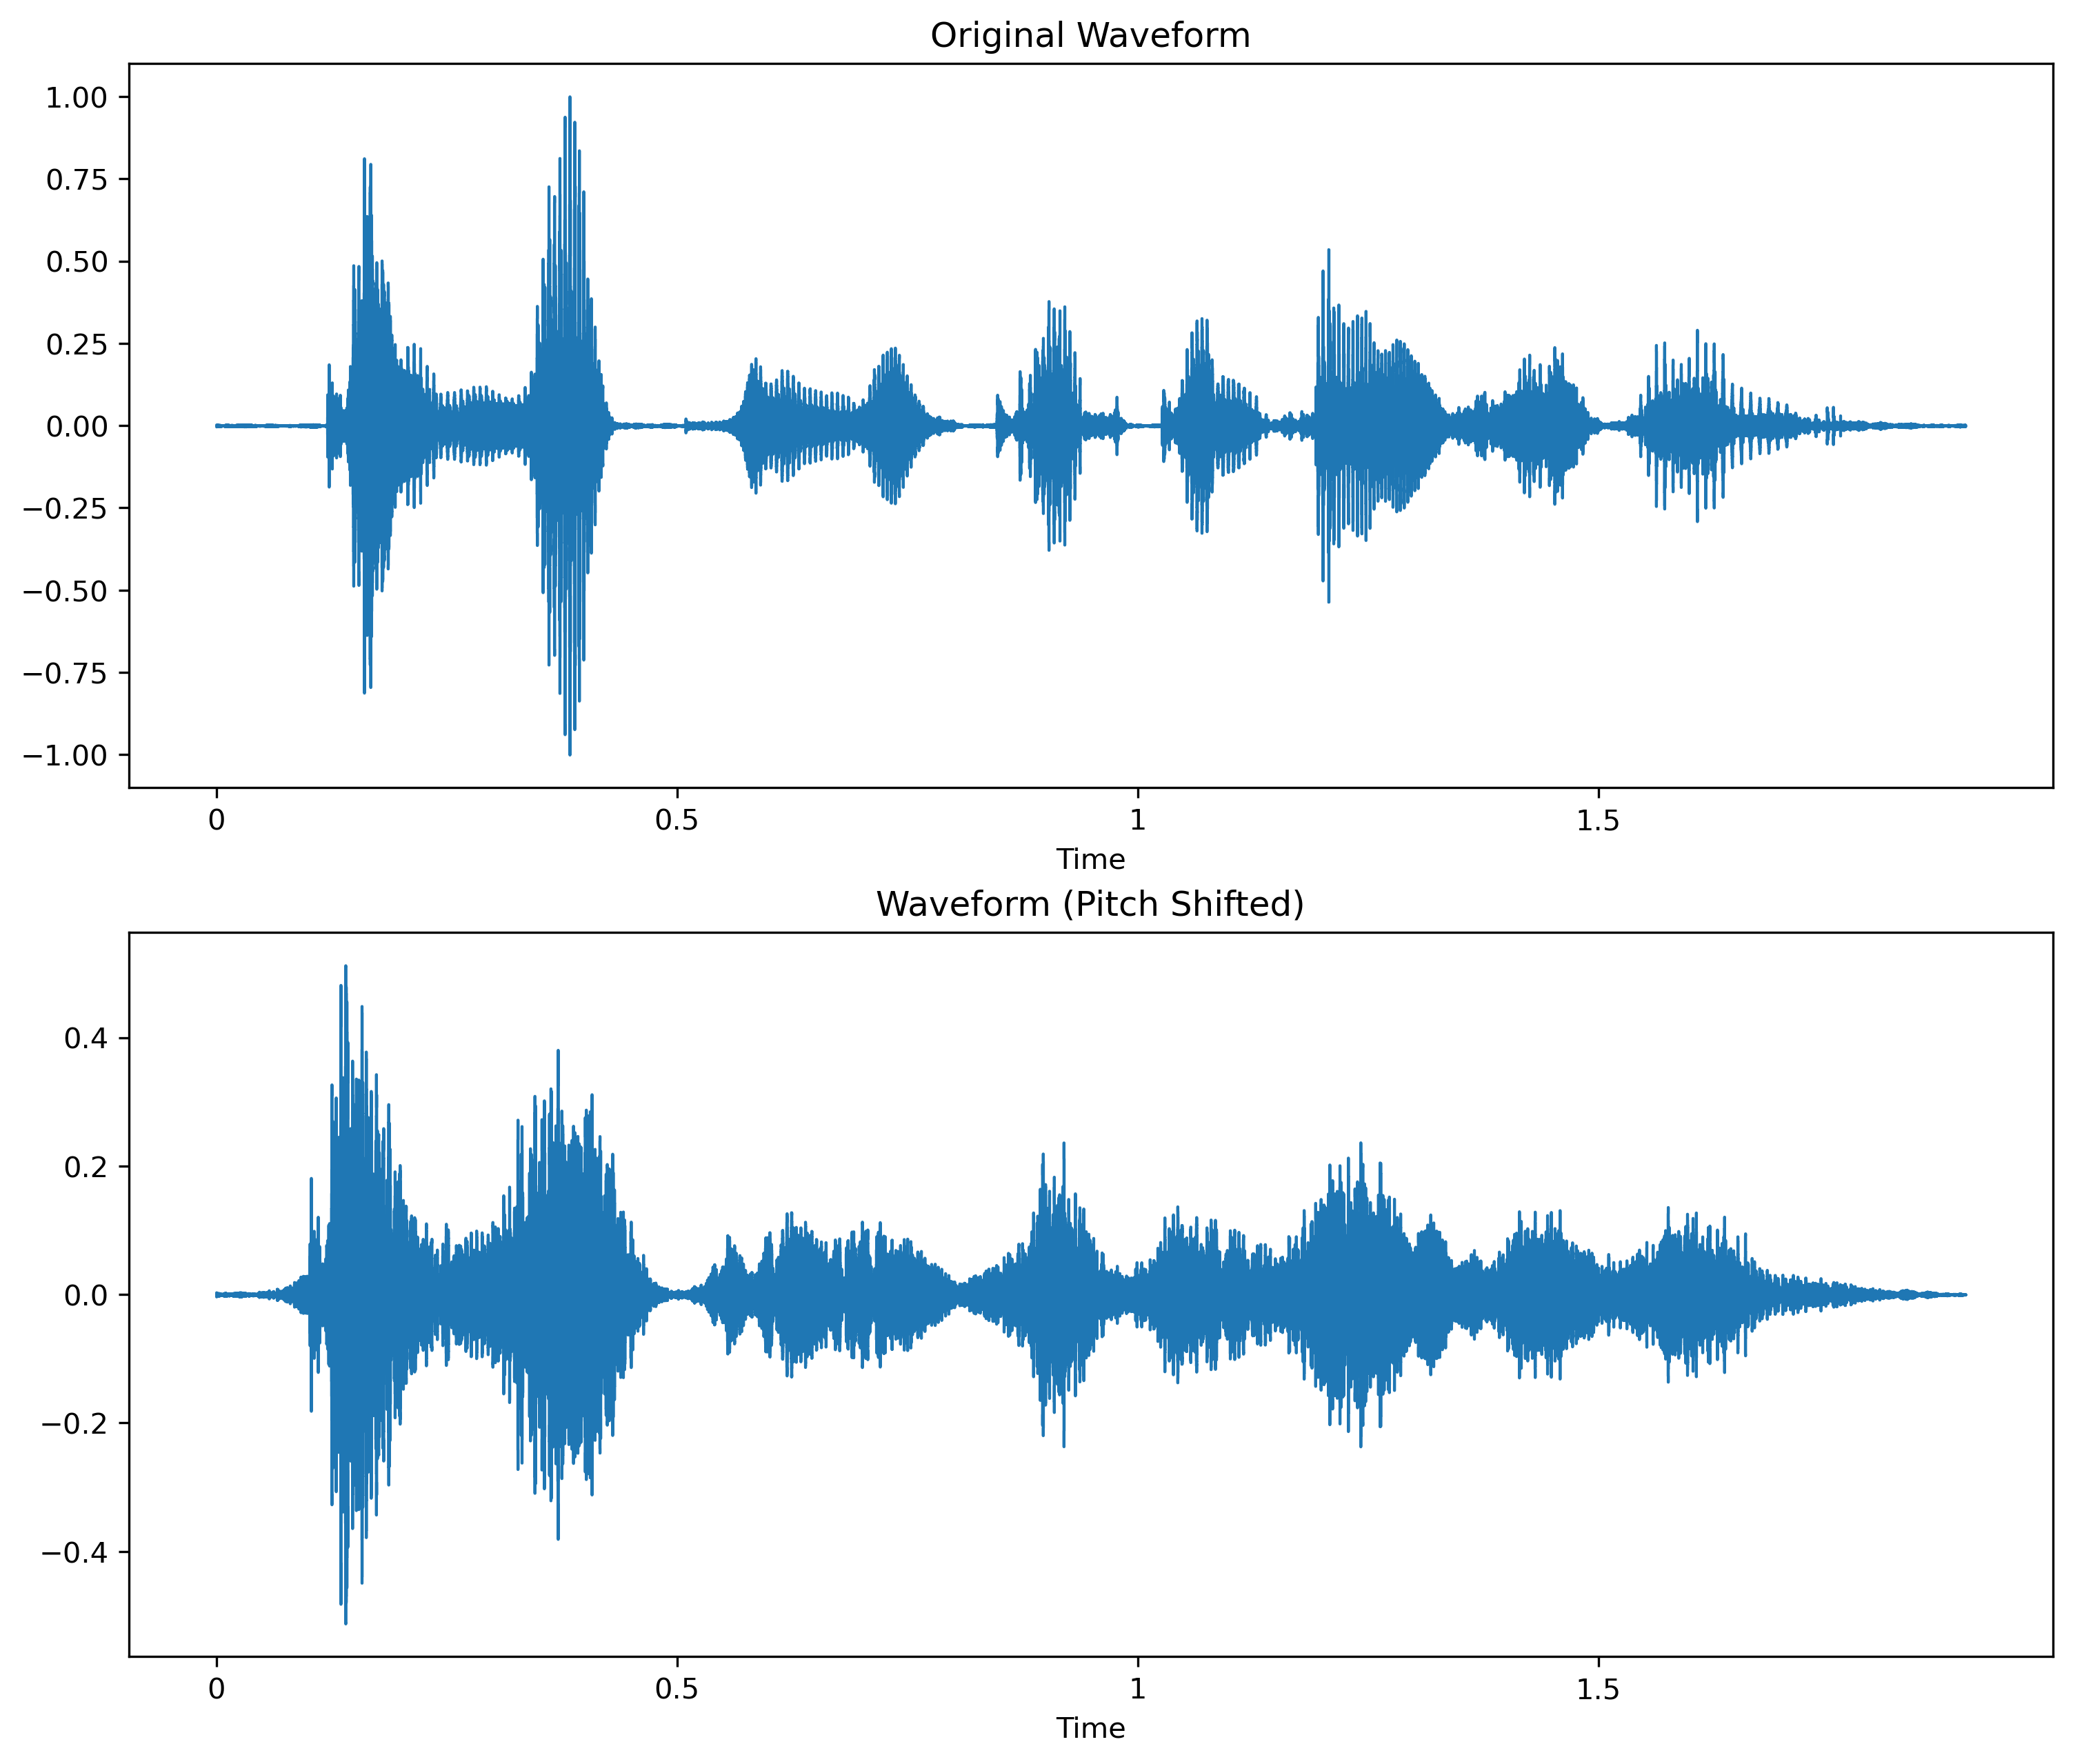
\includegraphics[width=0.7\linewidth]{../shift_ex.png}}
		\caption{نمونه از تغییر تن صدا}
		\label{fig:shift}
	\end{figure}
	\begin{figure}[!h]
		\centerline{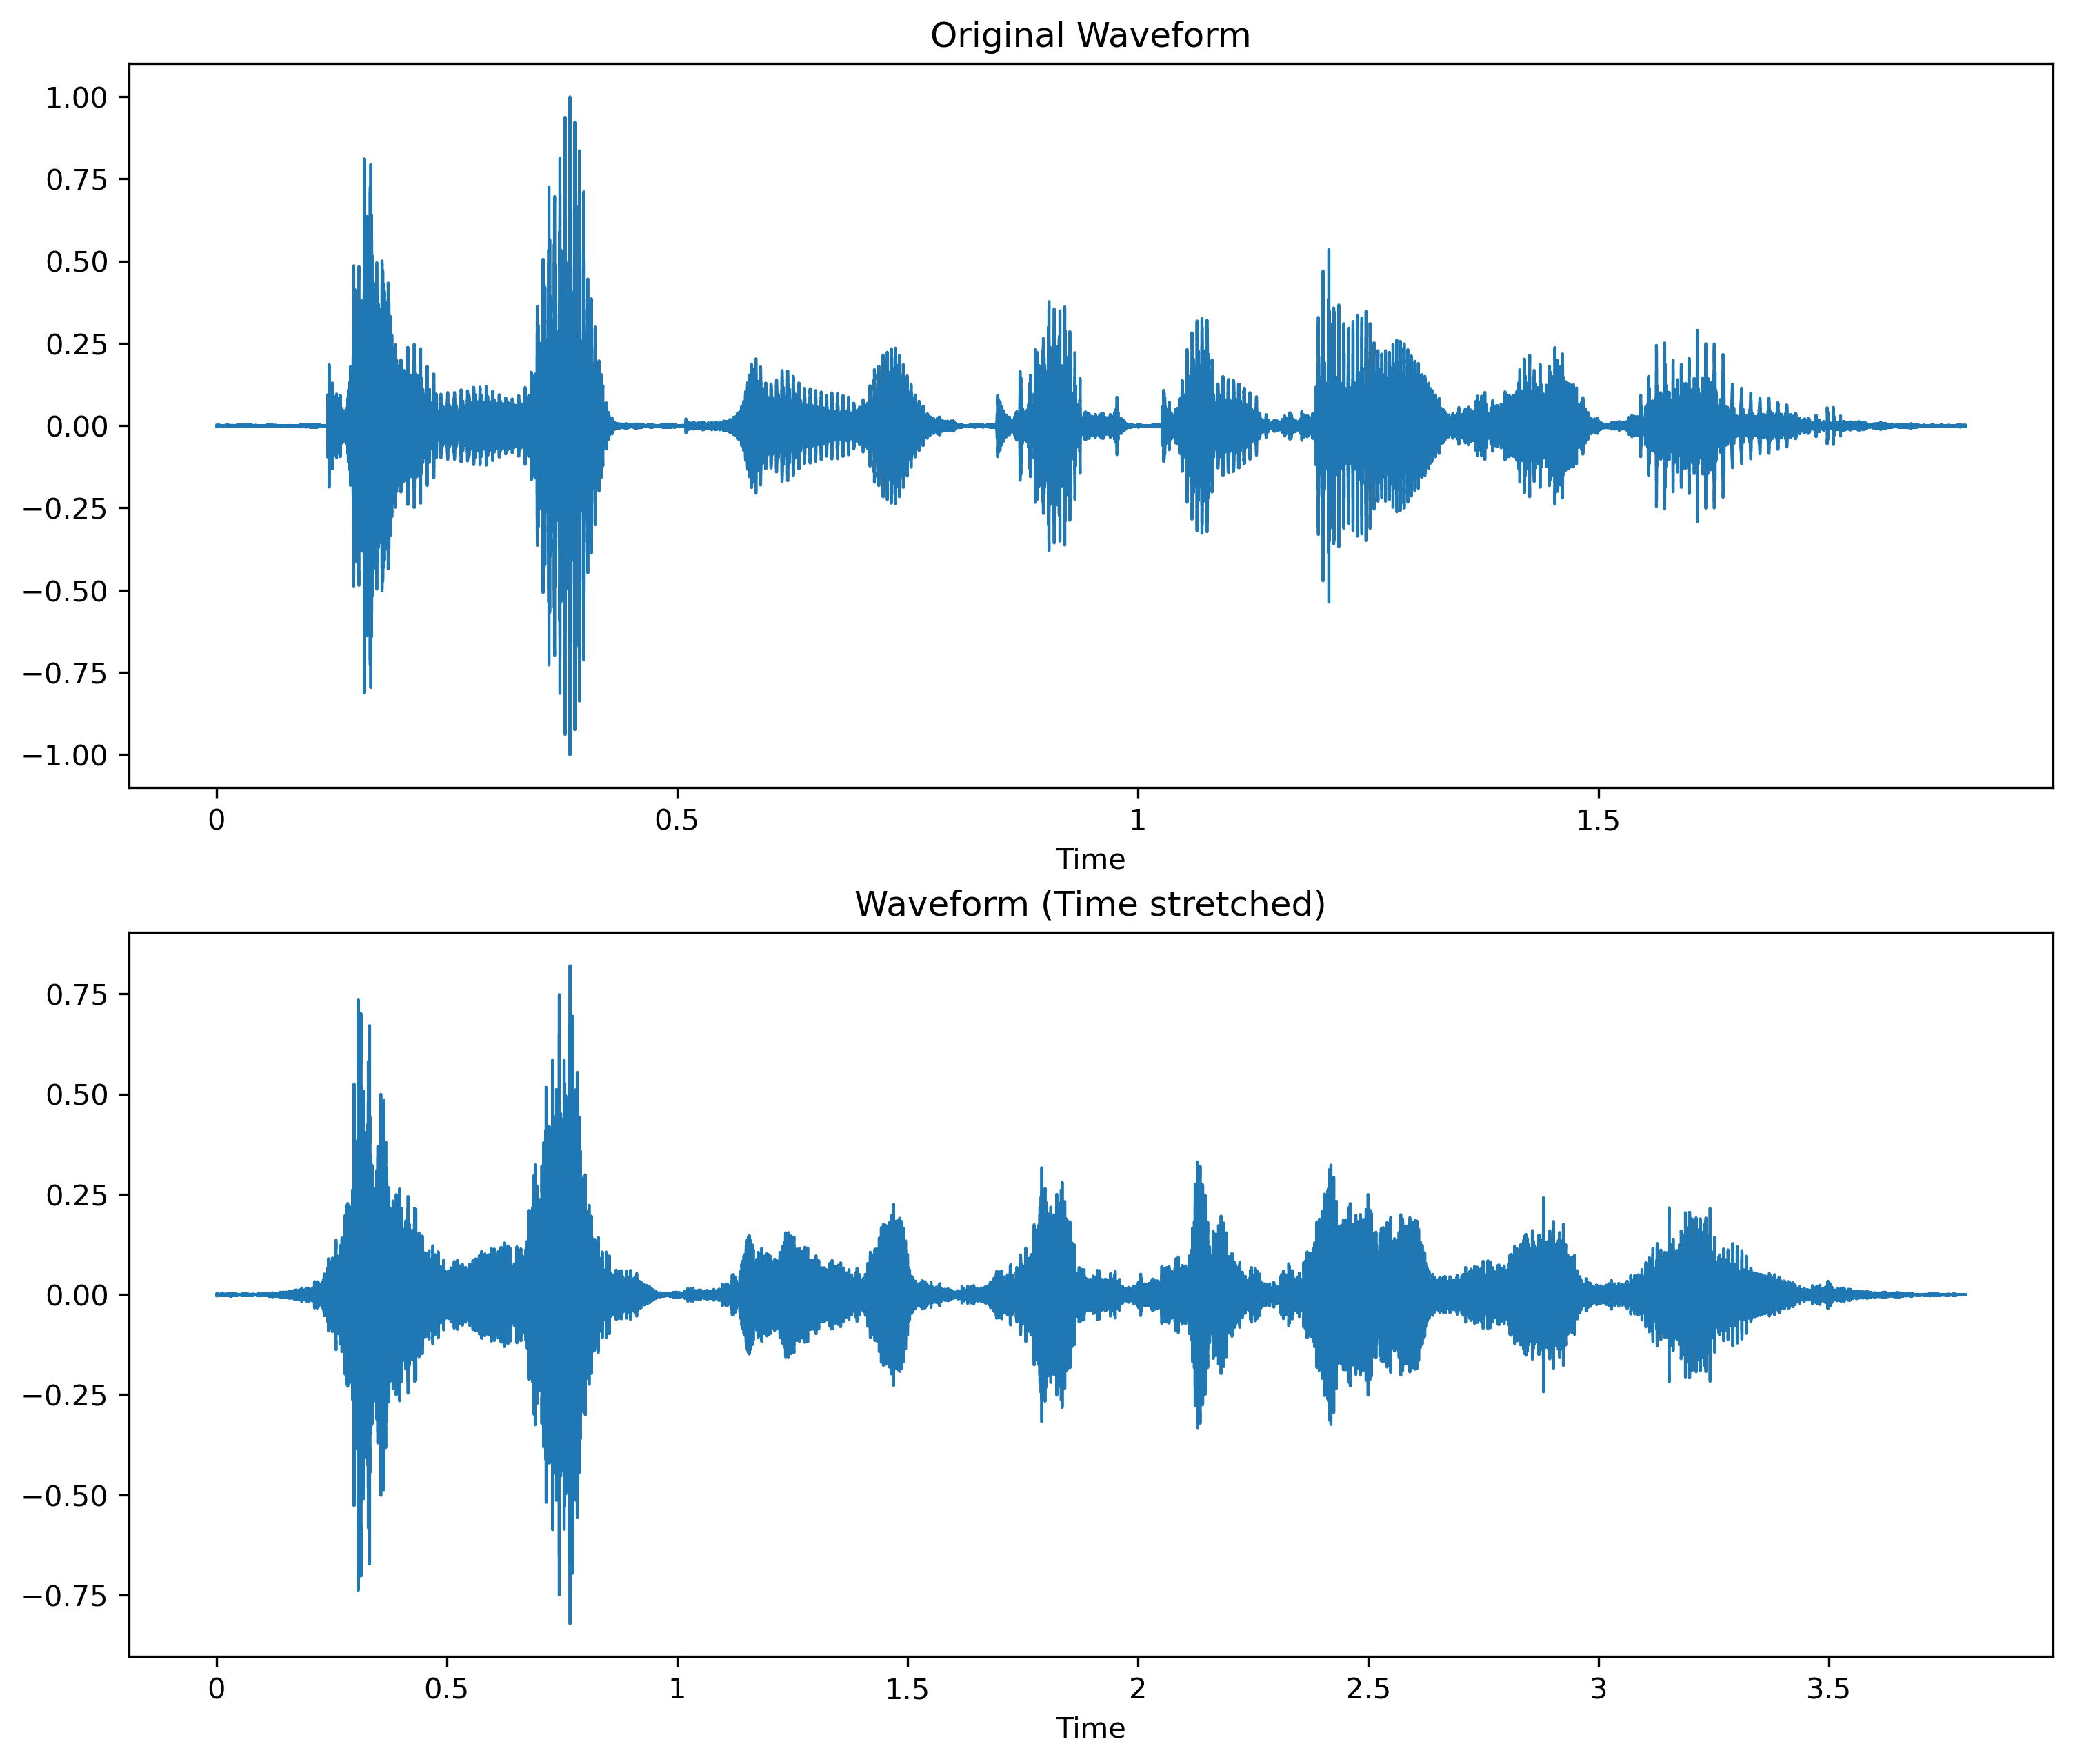
\includegraphics[width=0.7\linewidth]{../stretch_ex.png}}
		\caption{نمونه از تغییر سرعت گفتار}
		\label{fig:stretch}
	\end{figure}\\

	\section{پیش‌پردازش داده‌ها}
	در این قسمت با استفاده از داده‌های سری زمانی فایل‌های صوتی، ویژگی‌های 
	\lr{MFCC}
	\lr{(Mel-Frequency Cepstral Coefficients)}
	استخراج می‌شوند که بتوان آن‌ها را توسط شبکه پردازش کرد. این ویژگی‌ها شامل ۱۳ ویژگی هستند که در یک آرایه دو بعدی ذخیره می‌شوند. برای تولید این داده‌ها ابتدا نویز داده‌ها گرفته می‌شوند که می‌توان نمونه آن را در 
	\autoref{fig:noise}
	مشاهده کرد. سپس به دو راهی که در بخش گذشته توضیح داده شد داده‌ها افزوده شده و نهایتا 
	\lr{MFCC}
	آن‌ها استخراج می‌شود. این ویژگی‌ها در مرحله بعدی نرمال‌سازی می‌شوند که نتیجه آن در 
	\autoref{fig:MFCC_normalized}
	آمده است.
	\begin{figure}[!h]
		\centerline{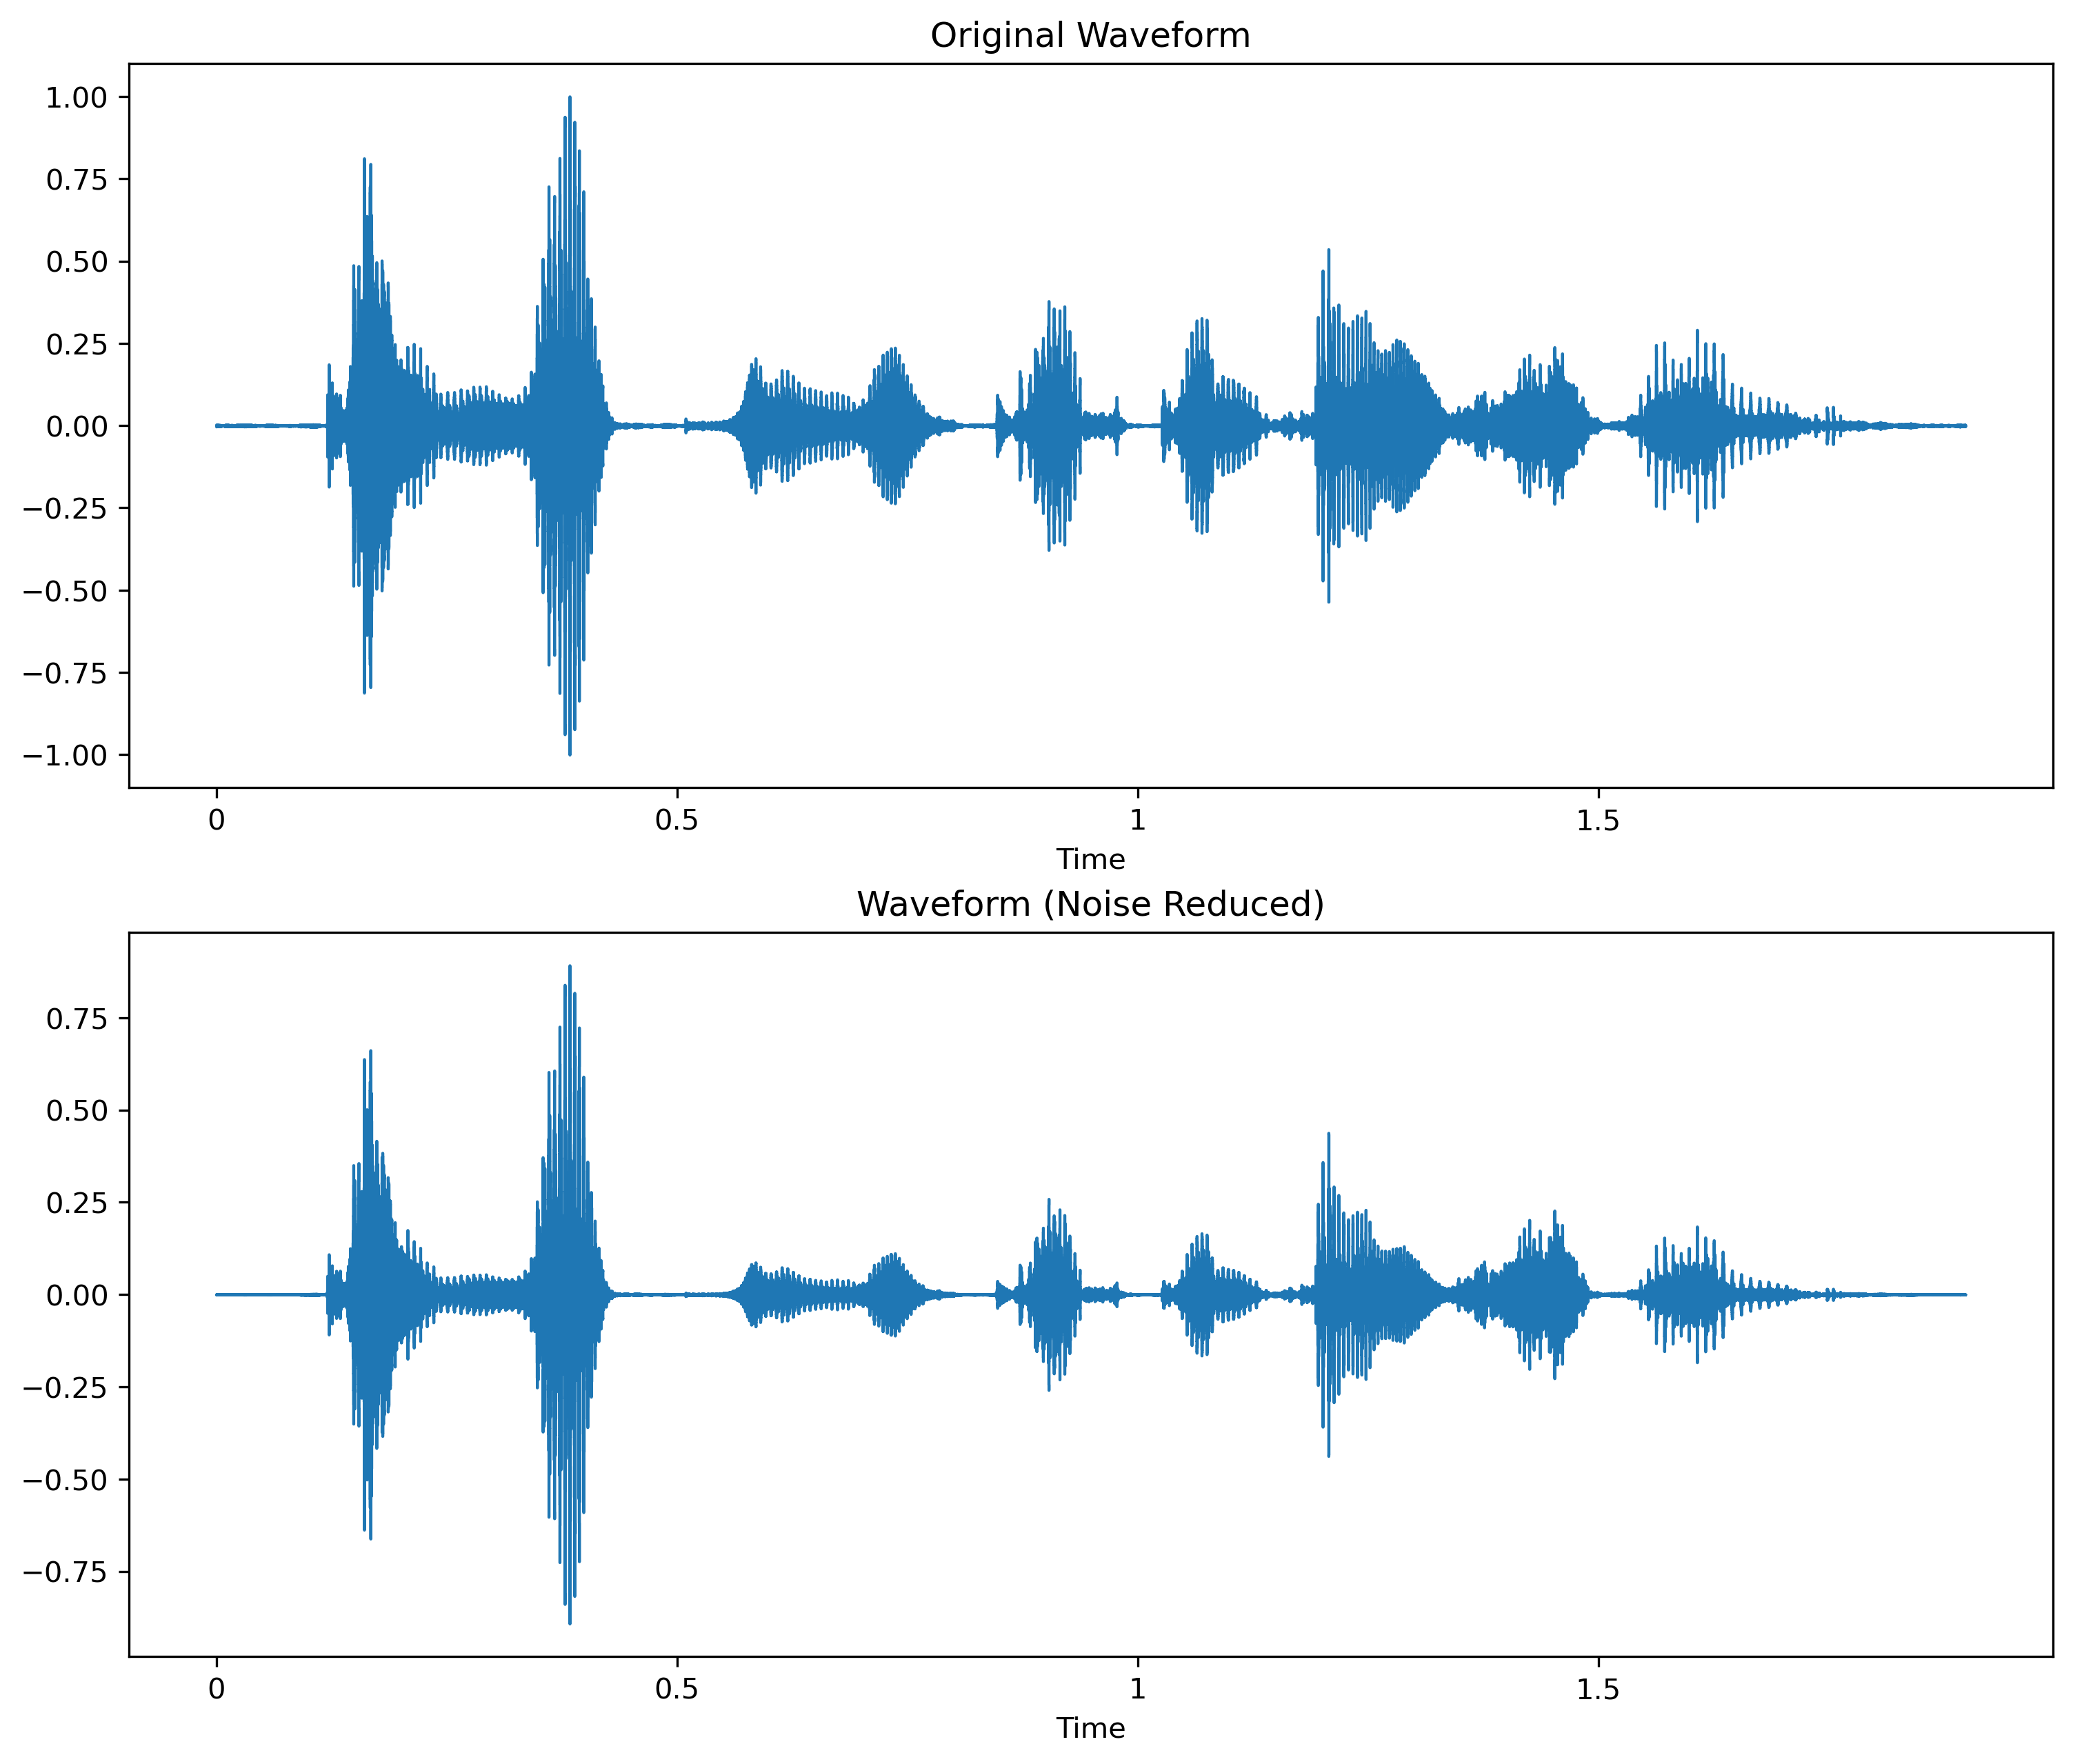
\includegraphics[width=0.8\linewidth]{../noise_ex.png}}
		\caption{نمونه از کم کردن نویز}
		\label{fig:noise}
	\end{figure}
	\begin{figure}[!h]
		\centerline{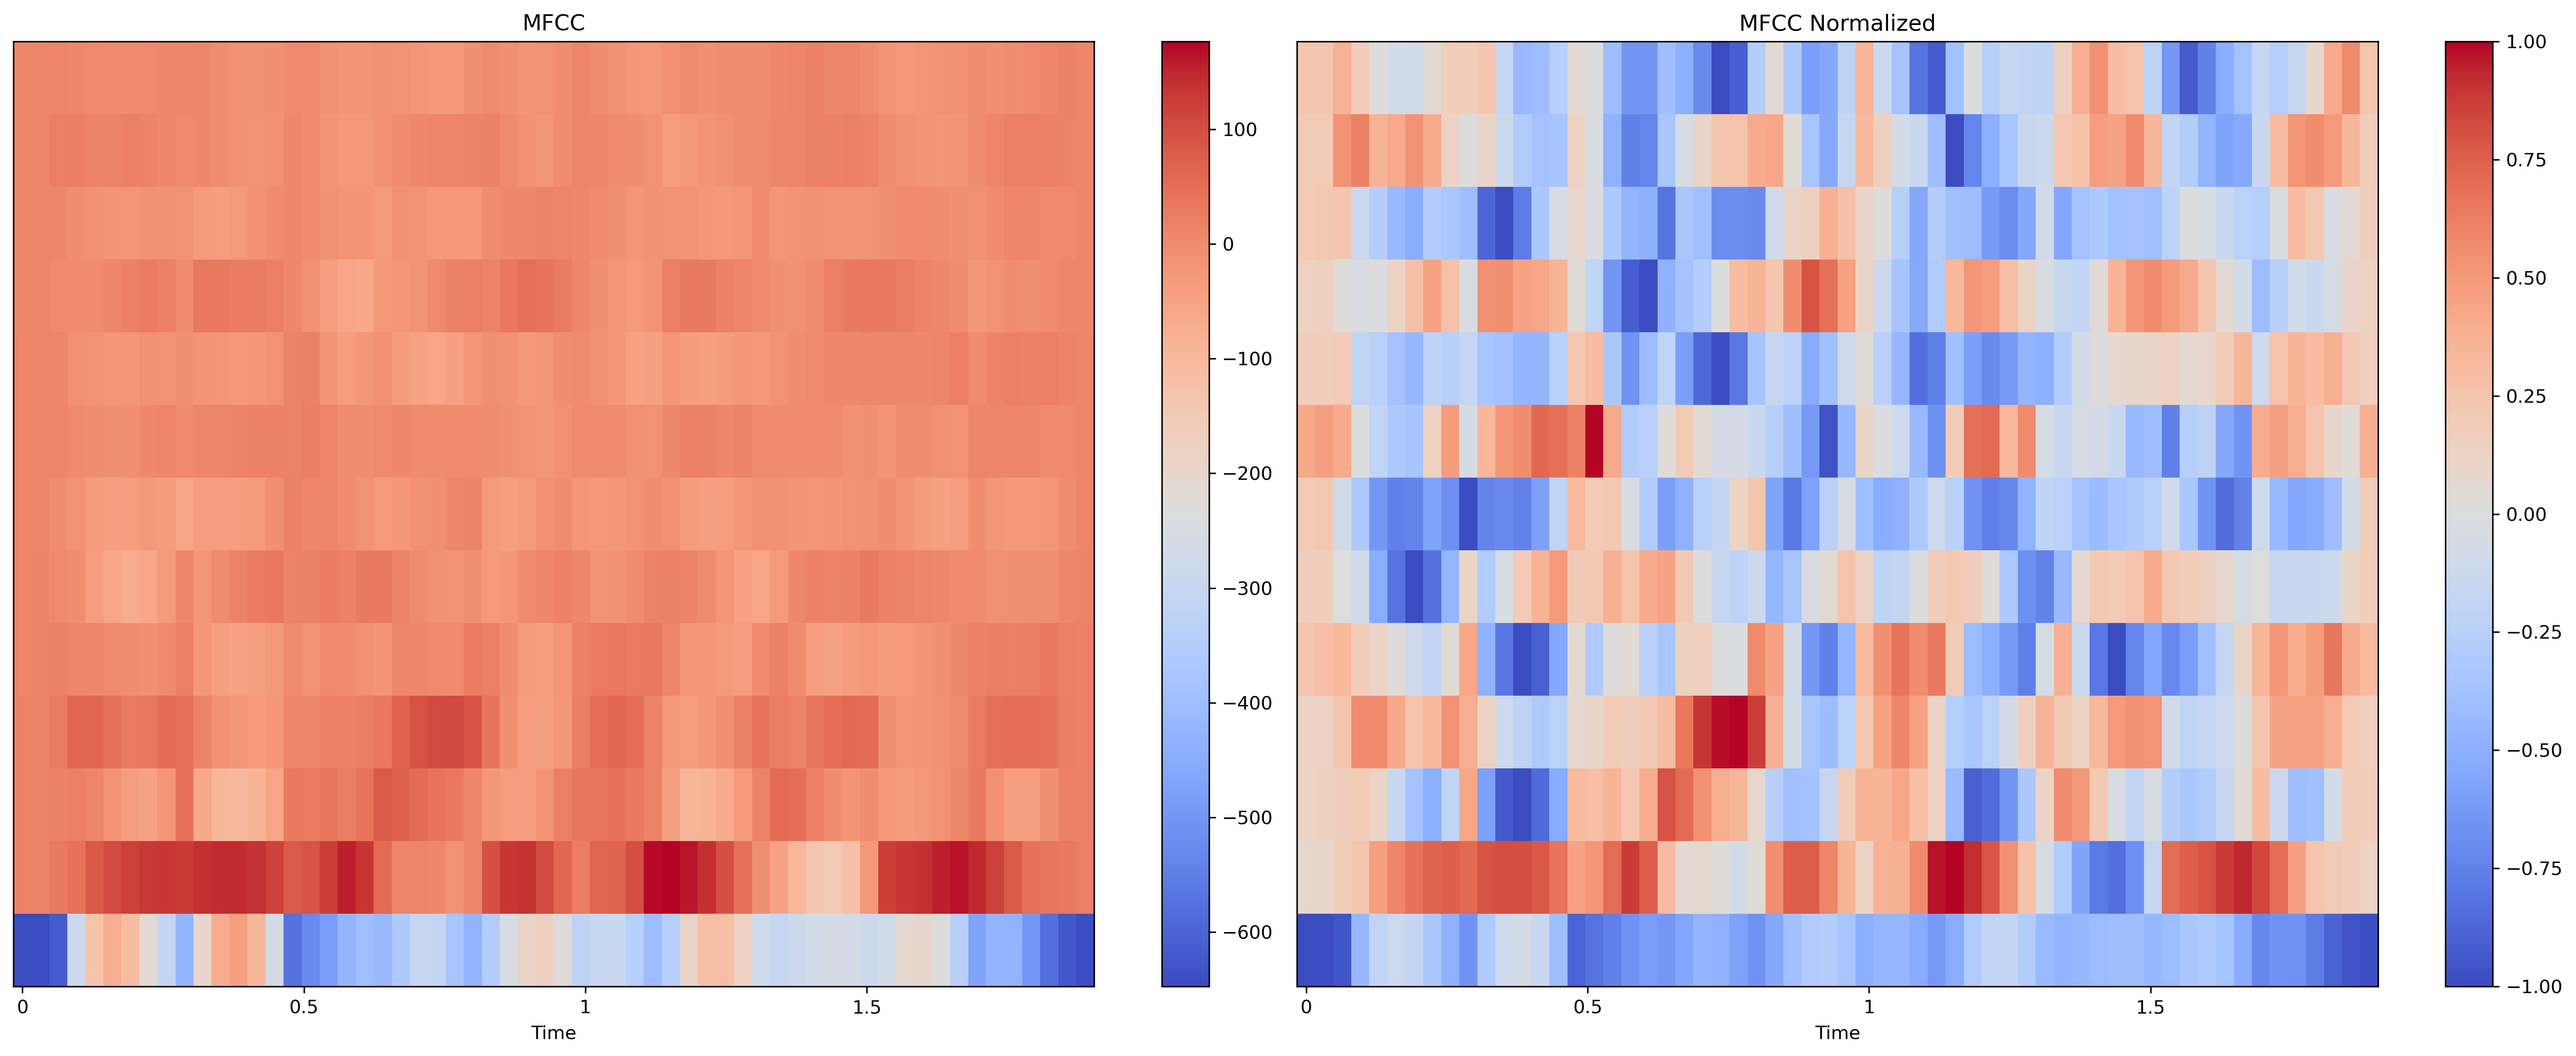
\includegraphics[width=1\linewidth]{../MFCC_ex.png}}
		\caption{نمونه از ویژگی‌های MFCC و نرمال‌سازی آن‌ها}
		\label{fig:MFCC_normalized}
	\end{figure}\\
	\clearpage
	\section{شبکه \lr{CNN}}
	برای پیش‌بینی در این قسمت از یک شبکه \lr{CNN} به ساختار 
	\autoref{fig:cnn_structure}
	استفاده می‌شود. این شبکه شامل لایه‌های پیچشی، انبایش، \lr{Dropout} برای جلوگیری از اورفیت شدن و دارای \lr{Batch Normalization} می‌باشد. ورودی شبکه به اندازه ویژگی‌های \lr{MFCC} به طول ۱۵۰ داده می‌باشد (۱۳ در ۱۵۰). تمامی لایه‌های پنهان دارای تابع فعال‌سازی \lr{Relu} بوده و لایه آخر از \lr{Softmax}استفاده می‌کند. برای تربیت مدل از الگوریتم \lr{Adam} با نرخ یادگیری $0.001$ استفاده می‌شود. حین تربیت از دو تابع هزینه مختلف استفاده شده که نتایج هریک در ادامه آمده است.\\
	\begin{figure}[htbp]
		\centerline{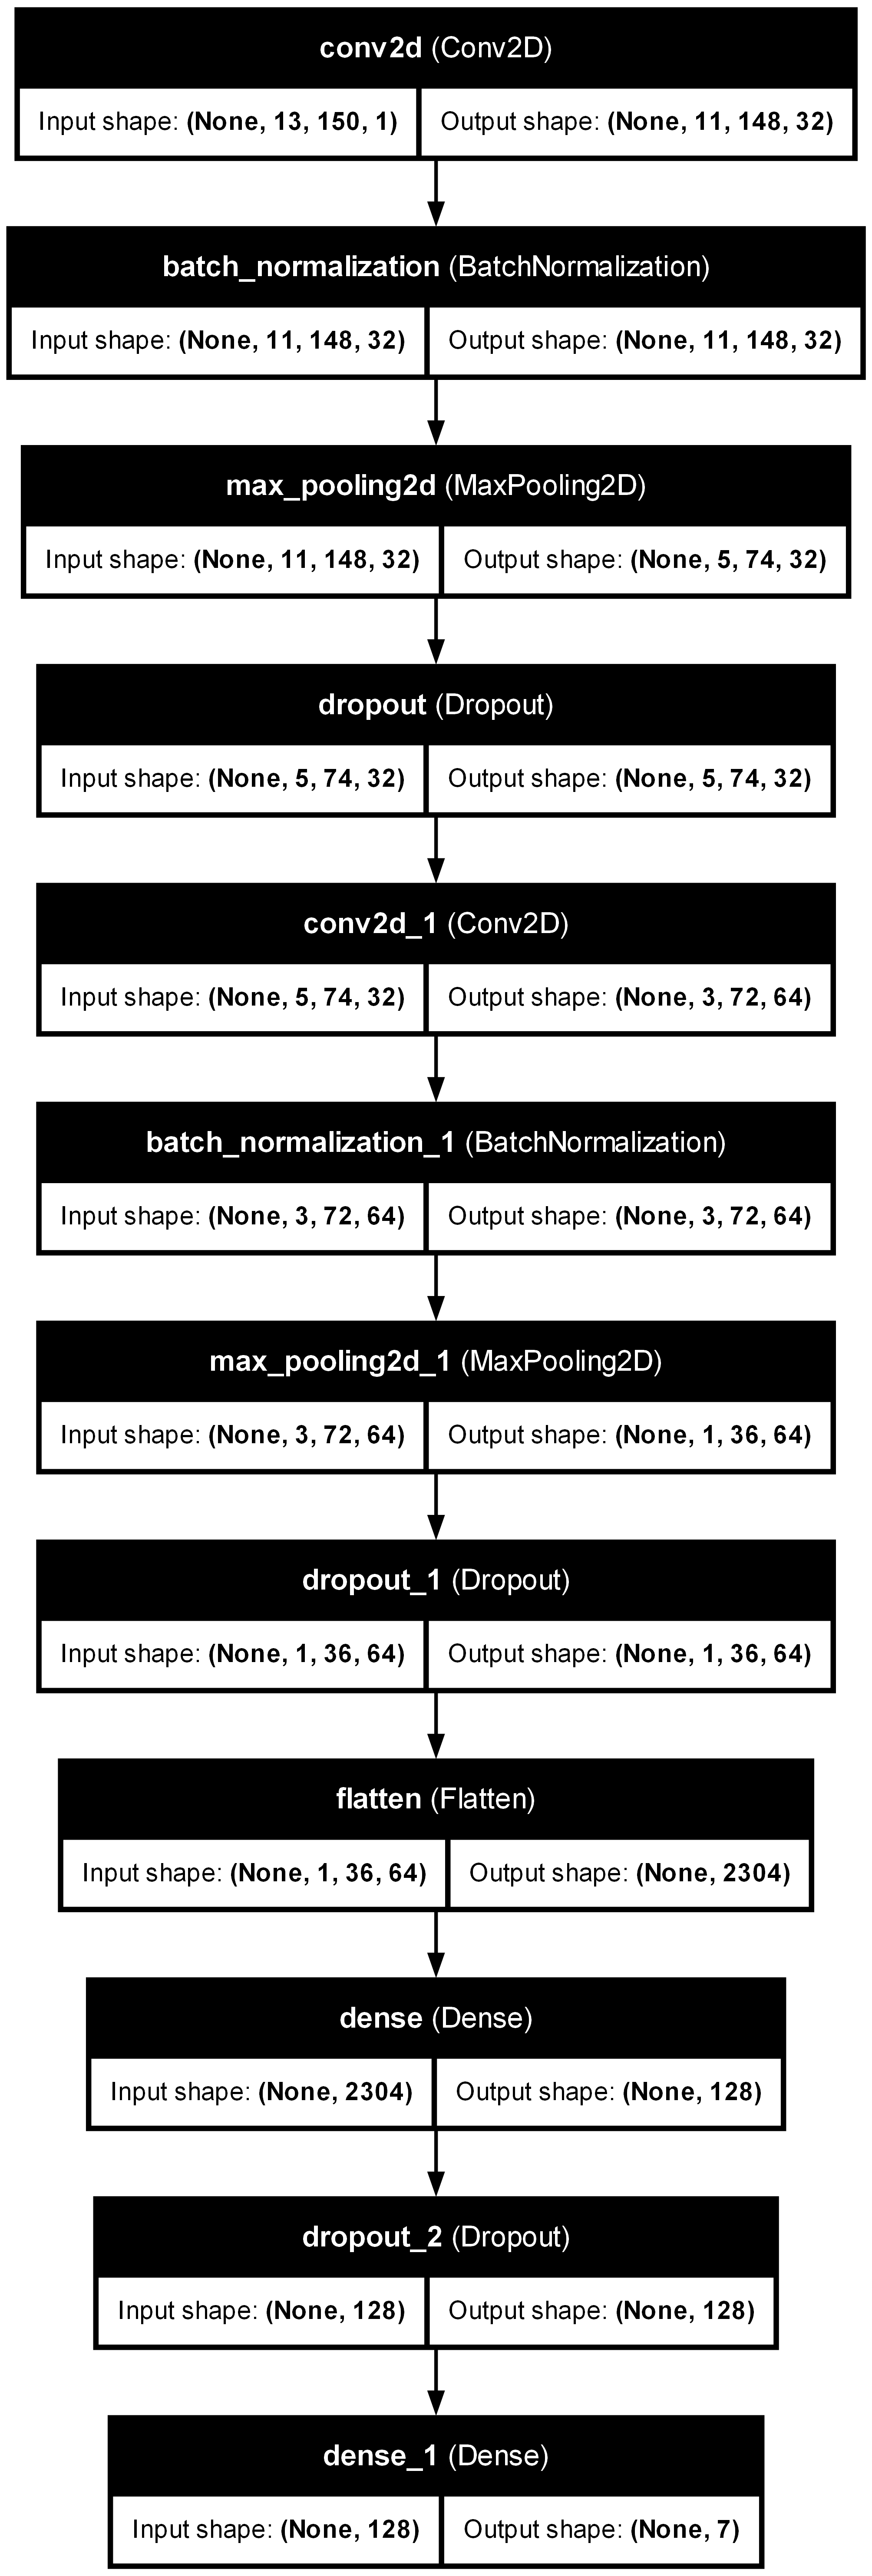
\includegraphics[width=0.3\linewidth]{../cnn_structure.png}}
		\caption{ساختار شبکه \lr{CNN}}
		\label{fig:cnn_structure}
	\end{figure}\\
	\begin{itemize}
		\item \textbf{\lr{Categorical Cross Entropy}}\\
		این تابع هزینه به صورت زیر می‌باشد:
		\begin{equation}
			L_{\text{CCE}} = -\sum_{i=1}^{C} y_i \log(\hat{y}_i)
		\end{equation}
		این تابع از پر استفاده‌ترین تابع هزینه برای شبکه‌های عصبی است و برای داده‌های \lr{One-Hot} استفاده می‌شود. این تابع برای مسائلی مناسب است که بیشتر از دو کلاس دارند. 
		\item \textbf{\lr{Kullback-Leibler Divergence}}\\
		این تابع هزینه به صورت زیر می‌باشد:
		\begin{equation}
			L_{\text{KL}} = \sum_{i=1}^{C} y_i \log\left(\frac{y_i}{\hat{y}_i}\right)
		\end{equation}
		مشابه تابع قبلی،‌ این تابع نیز برای مسائل چند کلاسه استفاده می‌شود. اما تفاوت ویژه‌ای که با آن دارن این است که برچسب‌ها لازم نیست به صورت \lr{One-Hot} باشند. این ویژگی به داده‌ها اجازه می‌دهد که عدم قطعیت داشته باشند. برای مثال در این مسئله چنانچه بتوان گفتار‌ها را در بیشتر از یک احساس دسته‌بندی کرد (برای مثال ۷۰ درصد خشم و ۳۰ درصد اضطراب) این تابع هزینه مفید خواهد بود. به این ترتیب حدس زده می‌شود که برای این مسئله کمی ضعیف‌تر از تابع \lr{Categorical Cross Entropy} عمل کند.
	\end{itemize}
	برای آموزش مدل از \lr{Early Stopping} با تحمل ۶ ایپاک استفاده می‌شود. بعد از تربیت مدل‌ها، دقت روی داده‌های تست برای مدل‌ها با تابع هزینه در جدول زیر آمده است
	\begin{table}[h!]
		\caption{جمع‌بندی دقت مدل‌ \lr{CNN} با دو تابع هزینه متفاوت}
		\begin{latin}
			\centering
			\begin{tabular}{|l|c|c|}
				\hline
				\textbf{Loss function} &  \textbf{Epochs till convergence} & \textbf{Test accuracy} \\ \hline
				Categorical Cross Entropy &  47 & 0.9163 \\  \hline
				Kullback-Leibler Divergence &  48 & 0.9003\\ \hline
			\end{tabular}
		\end{latin}
		\label{tab:accuracy_cnn} 
	\end{table}\\
	به این ترتیب تابع \lr{Categorical Cross Entropy} عملکرد بهتری هم در همگرایی و هم در دقت دارد. نمودار خطا و دقت مدل با این تابع هزینه در 
	\autoref{fig:cnn_loss1}
و ماتریس آشفتگی آن در 
	\autoref{fig:cnn_cm}
	آمده است.
		\begin{figure}[!h]
		\centerline{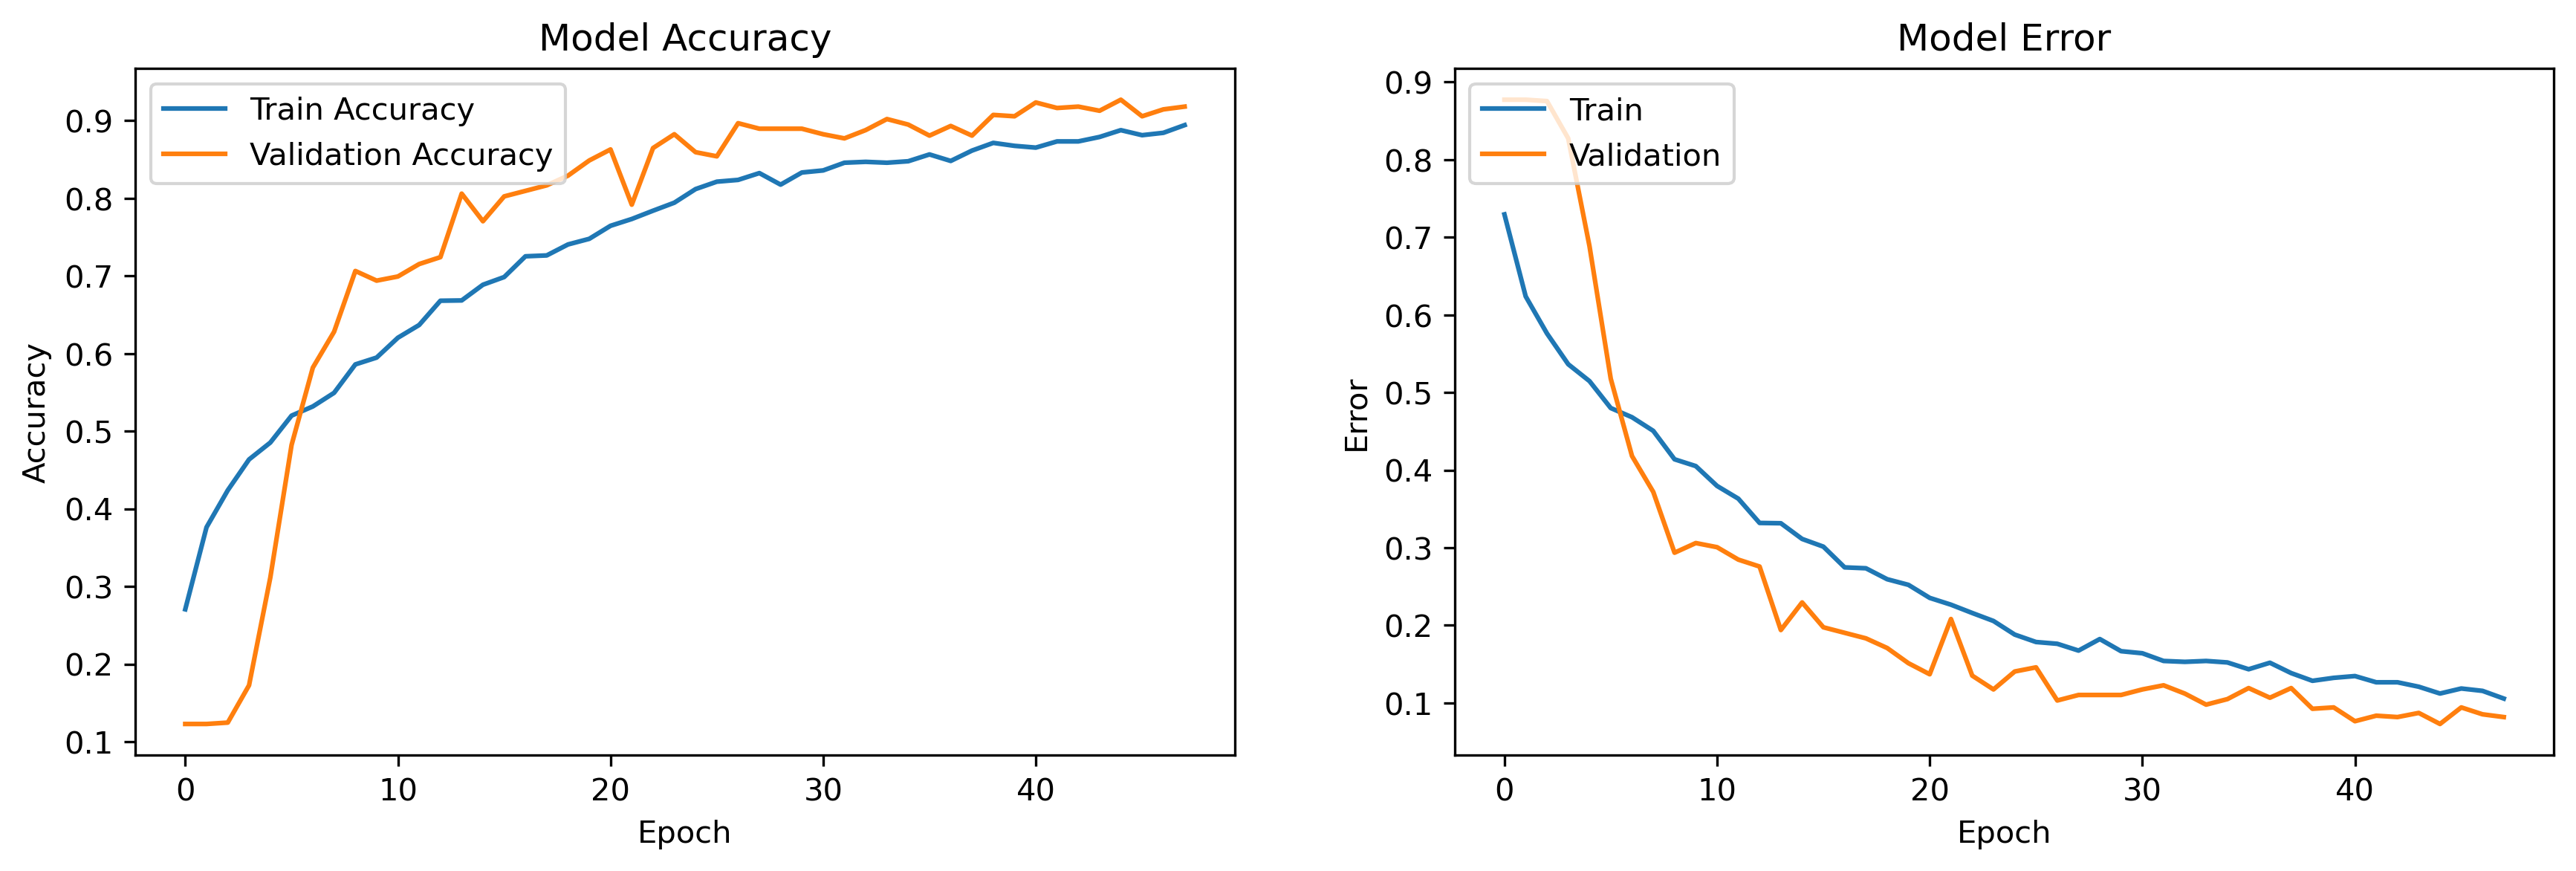
\includegraphics[width=1\linewidth]{../EMO_cnn_loss1.png}}
		\caption{نمودار خطا و دقت  -  مدل \lr{CNN}}
		\label{fig:cnn_loss1}
	\end{figure}
	\begin{figure}[!h]
		\centerline{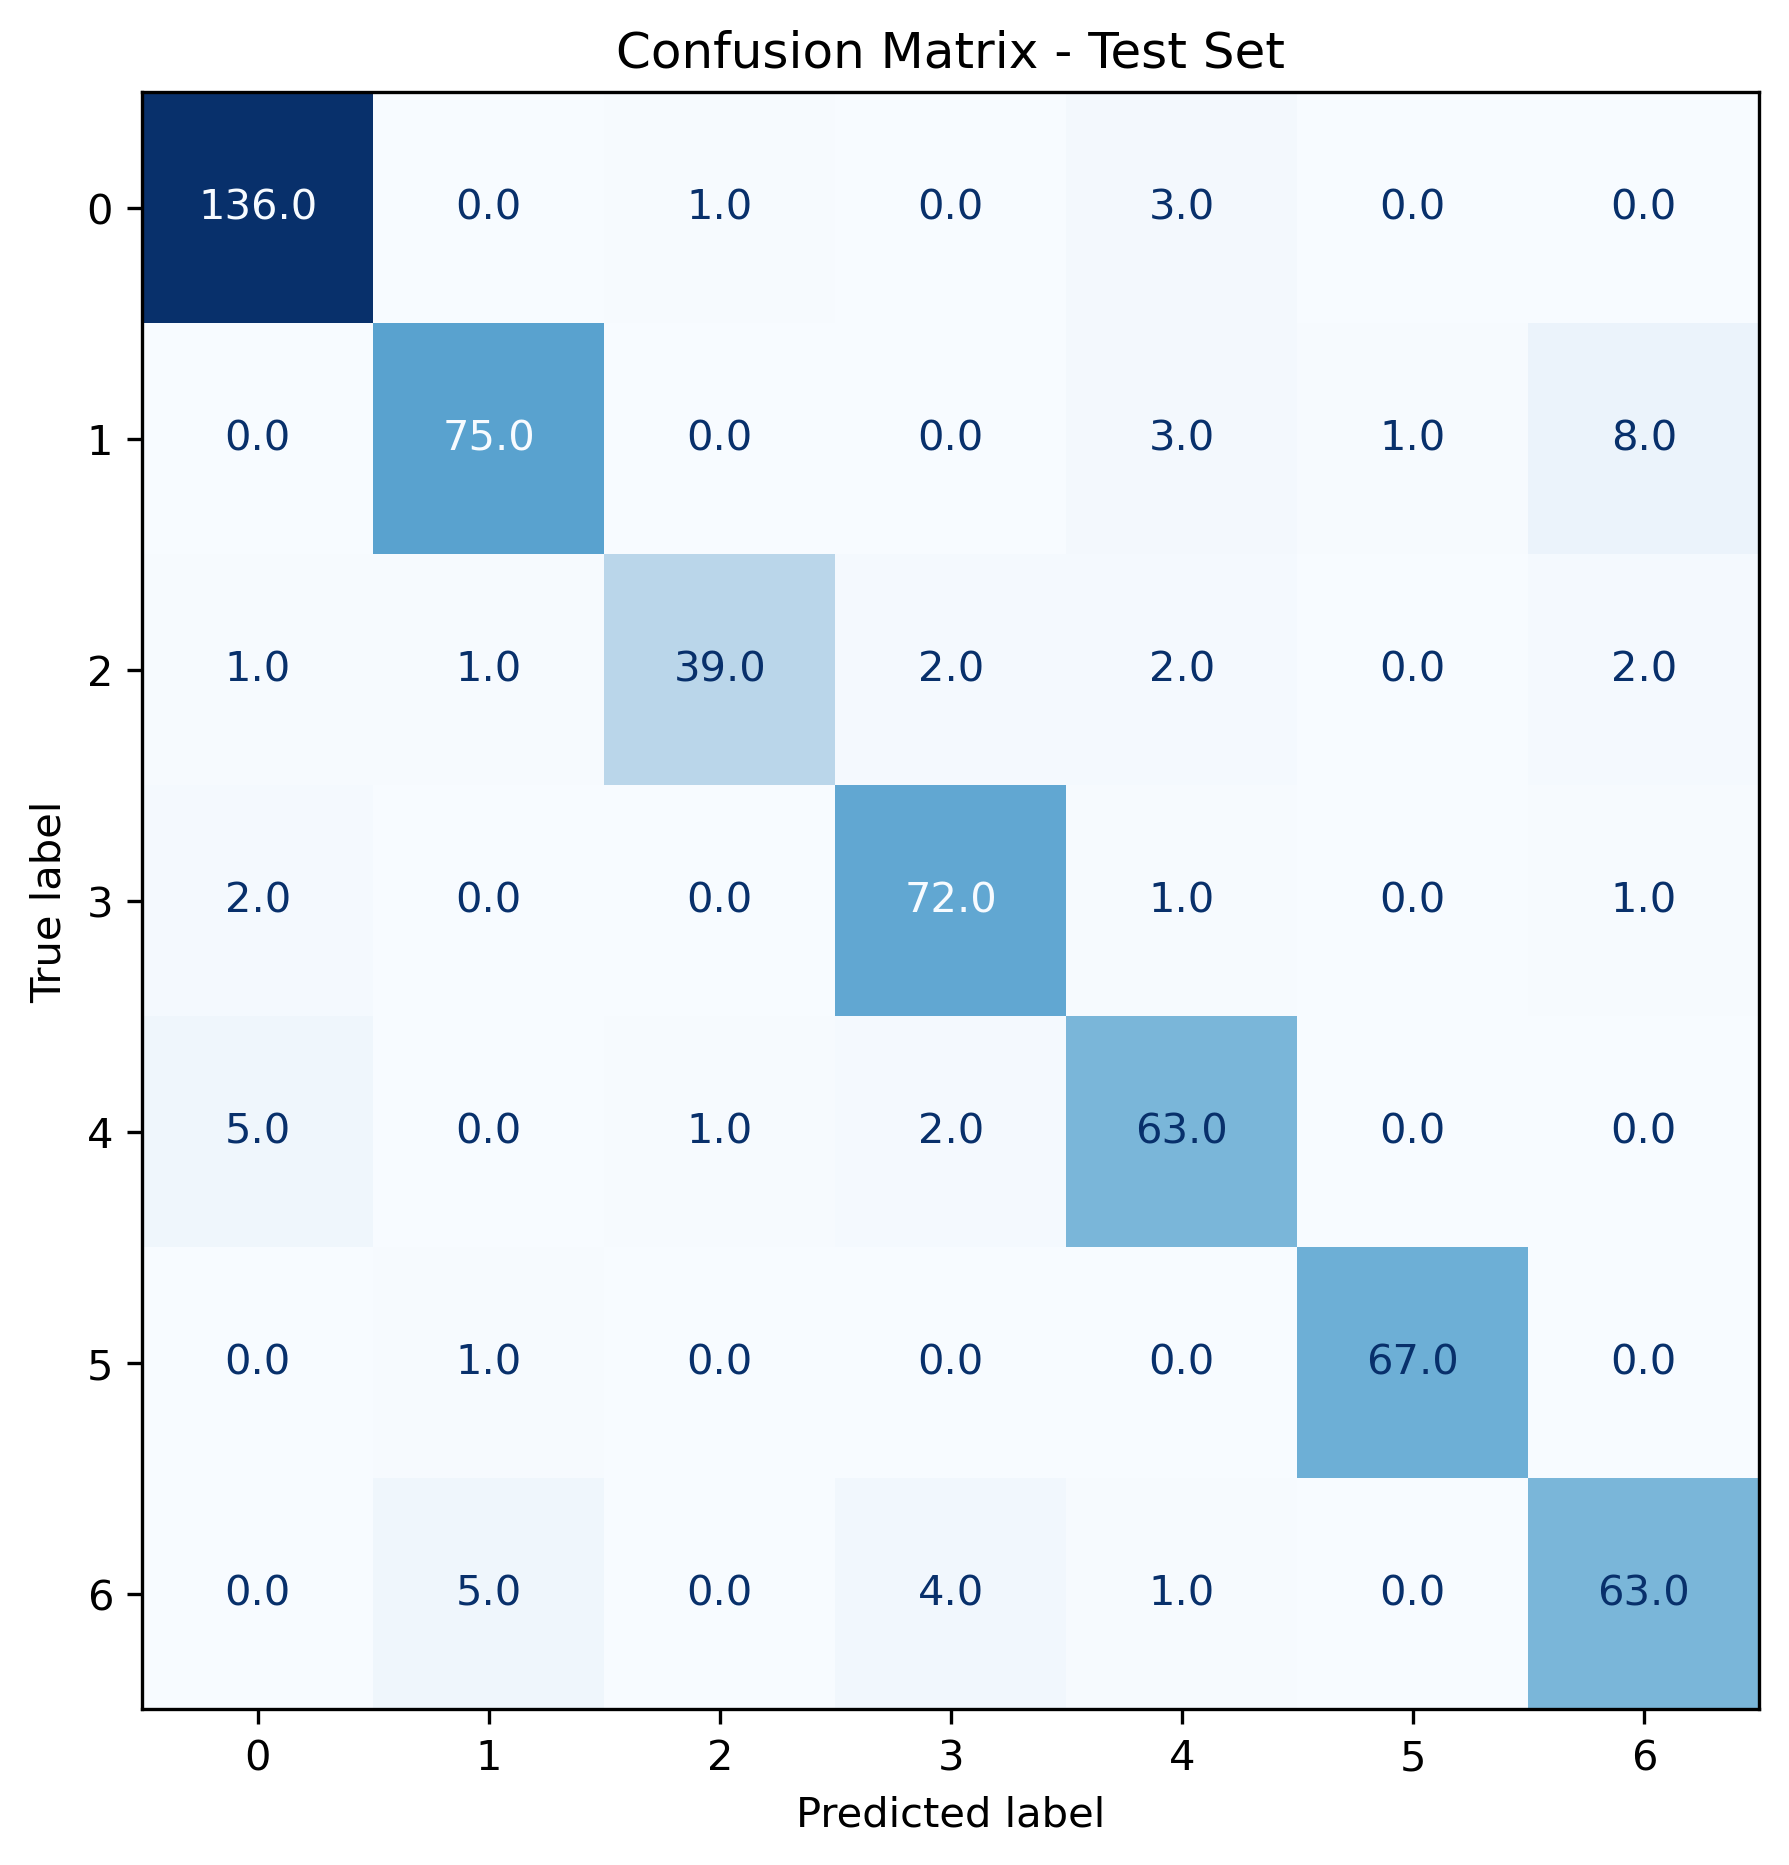
\includegraphics[width=0.7\linewidth]{../cnn_loss1_cm.png}}
		\caption{ماتریس آشفتگی - مدل \lr{CNN}}
		\label{fig:cnn_cm} 
	\end{figure}\\
	می‌توان در ماتریس آشفتگی مشاهده‌ کرد که مدل دقت نسبتا خوبی داشته و اکثر کلاس‌ها به درستی پیش‌بینی می‌شوند. طبیعتا درصد دقت در کلاس‌هایی که داده‌ها در آن کمتر است، هم به دلیل تربیت ضعیف‌تر و هم به علت نسبت بالاتر خطا‌ها، پایین‌تر می‌آید. همچنین می‌توان دید که کلاس‌هایی که برای انسان نیز شبیه به هم هستند با هم بیشتر اشتباه گرفته می‌شوند. برای مثال بی‌حوصلگی (کلاس ۱) و بی‌تفاوتی (کلاس ۶) بیشتر از سایر داده‌ها به جای هم تشخیص داده شده‌اند.
	\clearpage
	\section{شبکه \lr{CNN - LSTM}}
	در این بخش از یک شبکه \lr{LSTM} استفاده می‌شود که برای کاهش ابعادی، شبکه \lr{CNN} بخش قبلی به آن اضافه شده است. به این ترتیب ساختار شبکه تقریبا همان 
	\autoref{fig:cnn_structure}
	می‌باشد. با این تفاوت که بعد از آخرین لایه پیچشی و انبایشی،‌ یک شبکه \lr{LSTM} وجود دارد که در نهایت به سایر لایه‌های شبکه متصل می‌شود. دقت مدل به ازای دو تابع هزینه مختلف توضیح داده شده به صورت زیر می‌باشد که باز هم تابع اول بهتر عمل می‌کند.
	  
	\begin{table}[h!]
		\caption{جمع‌بندی دقت مدل‌ \lr{CNN-LSTM} با دو تابع هزینه متفاوت}
		\begin{latin}
			\centering
			\begin{tabular}{|l|c|c|}
				\hline
				\textbf{Loss function} &  \textbf{Epochs till convergence} & \textbf{Test accuracy} \\ \hline
				Categorical Cross Entropy &  37 & 0.9306 \\  \hline
				Kullback-Leibler Divergence &  35 & 0.9074\\ \hline
			\end{tabular}
		\end{latin}
		\label{tab:accuracy_cnnlstm} 
 	\end{table}
	نمودار خطا و دقت در
	\autoref{fig:cnn_loss1}
	و ماتریس آشفتگی آن در 
	\autoref{fig:cnn_cm}
	آمده است.
	\begin{figure}[!h]
		\centerline{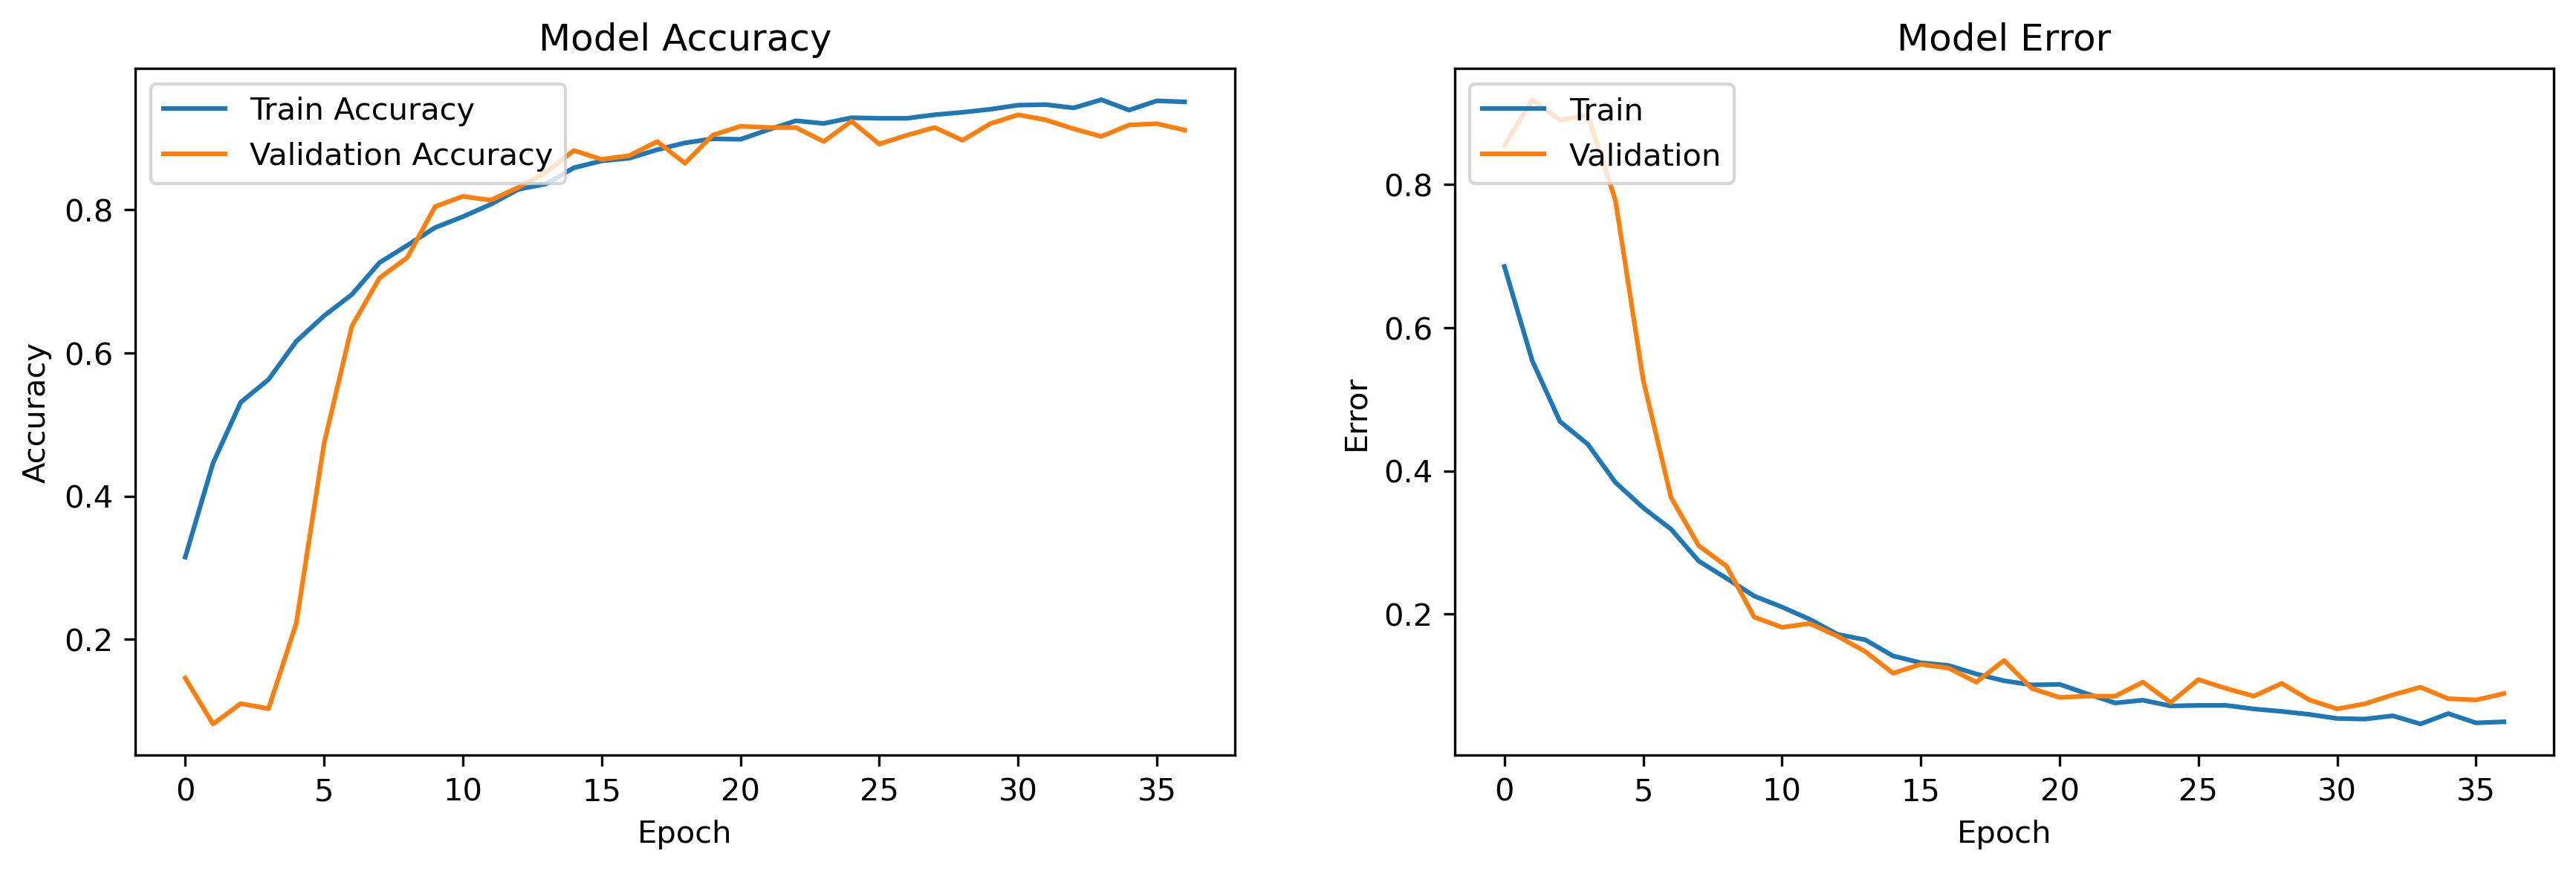
\includegraphics[width=1\linewidth]{../EMO_cnnlstm_loss1.png}}
		\caption{نمودار خطا و دقت  -  مدل \lr{CNN-LSTM}}
		\label{fig:cnnlstm_loss1}
	\end{figure}
	\begin{figure}[!h]
		\centerline{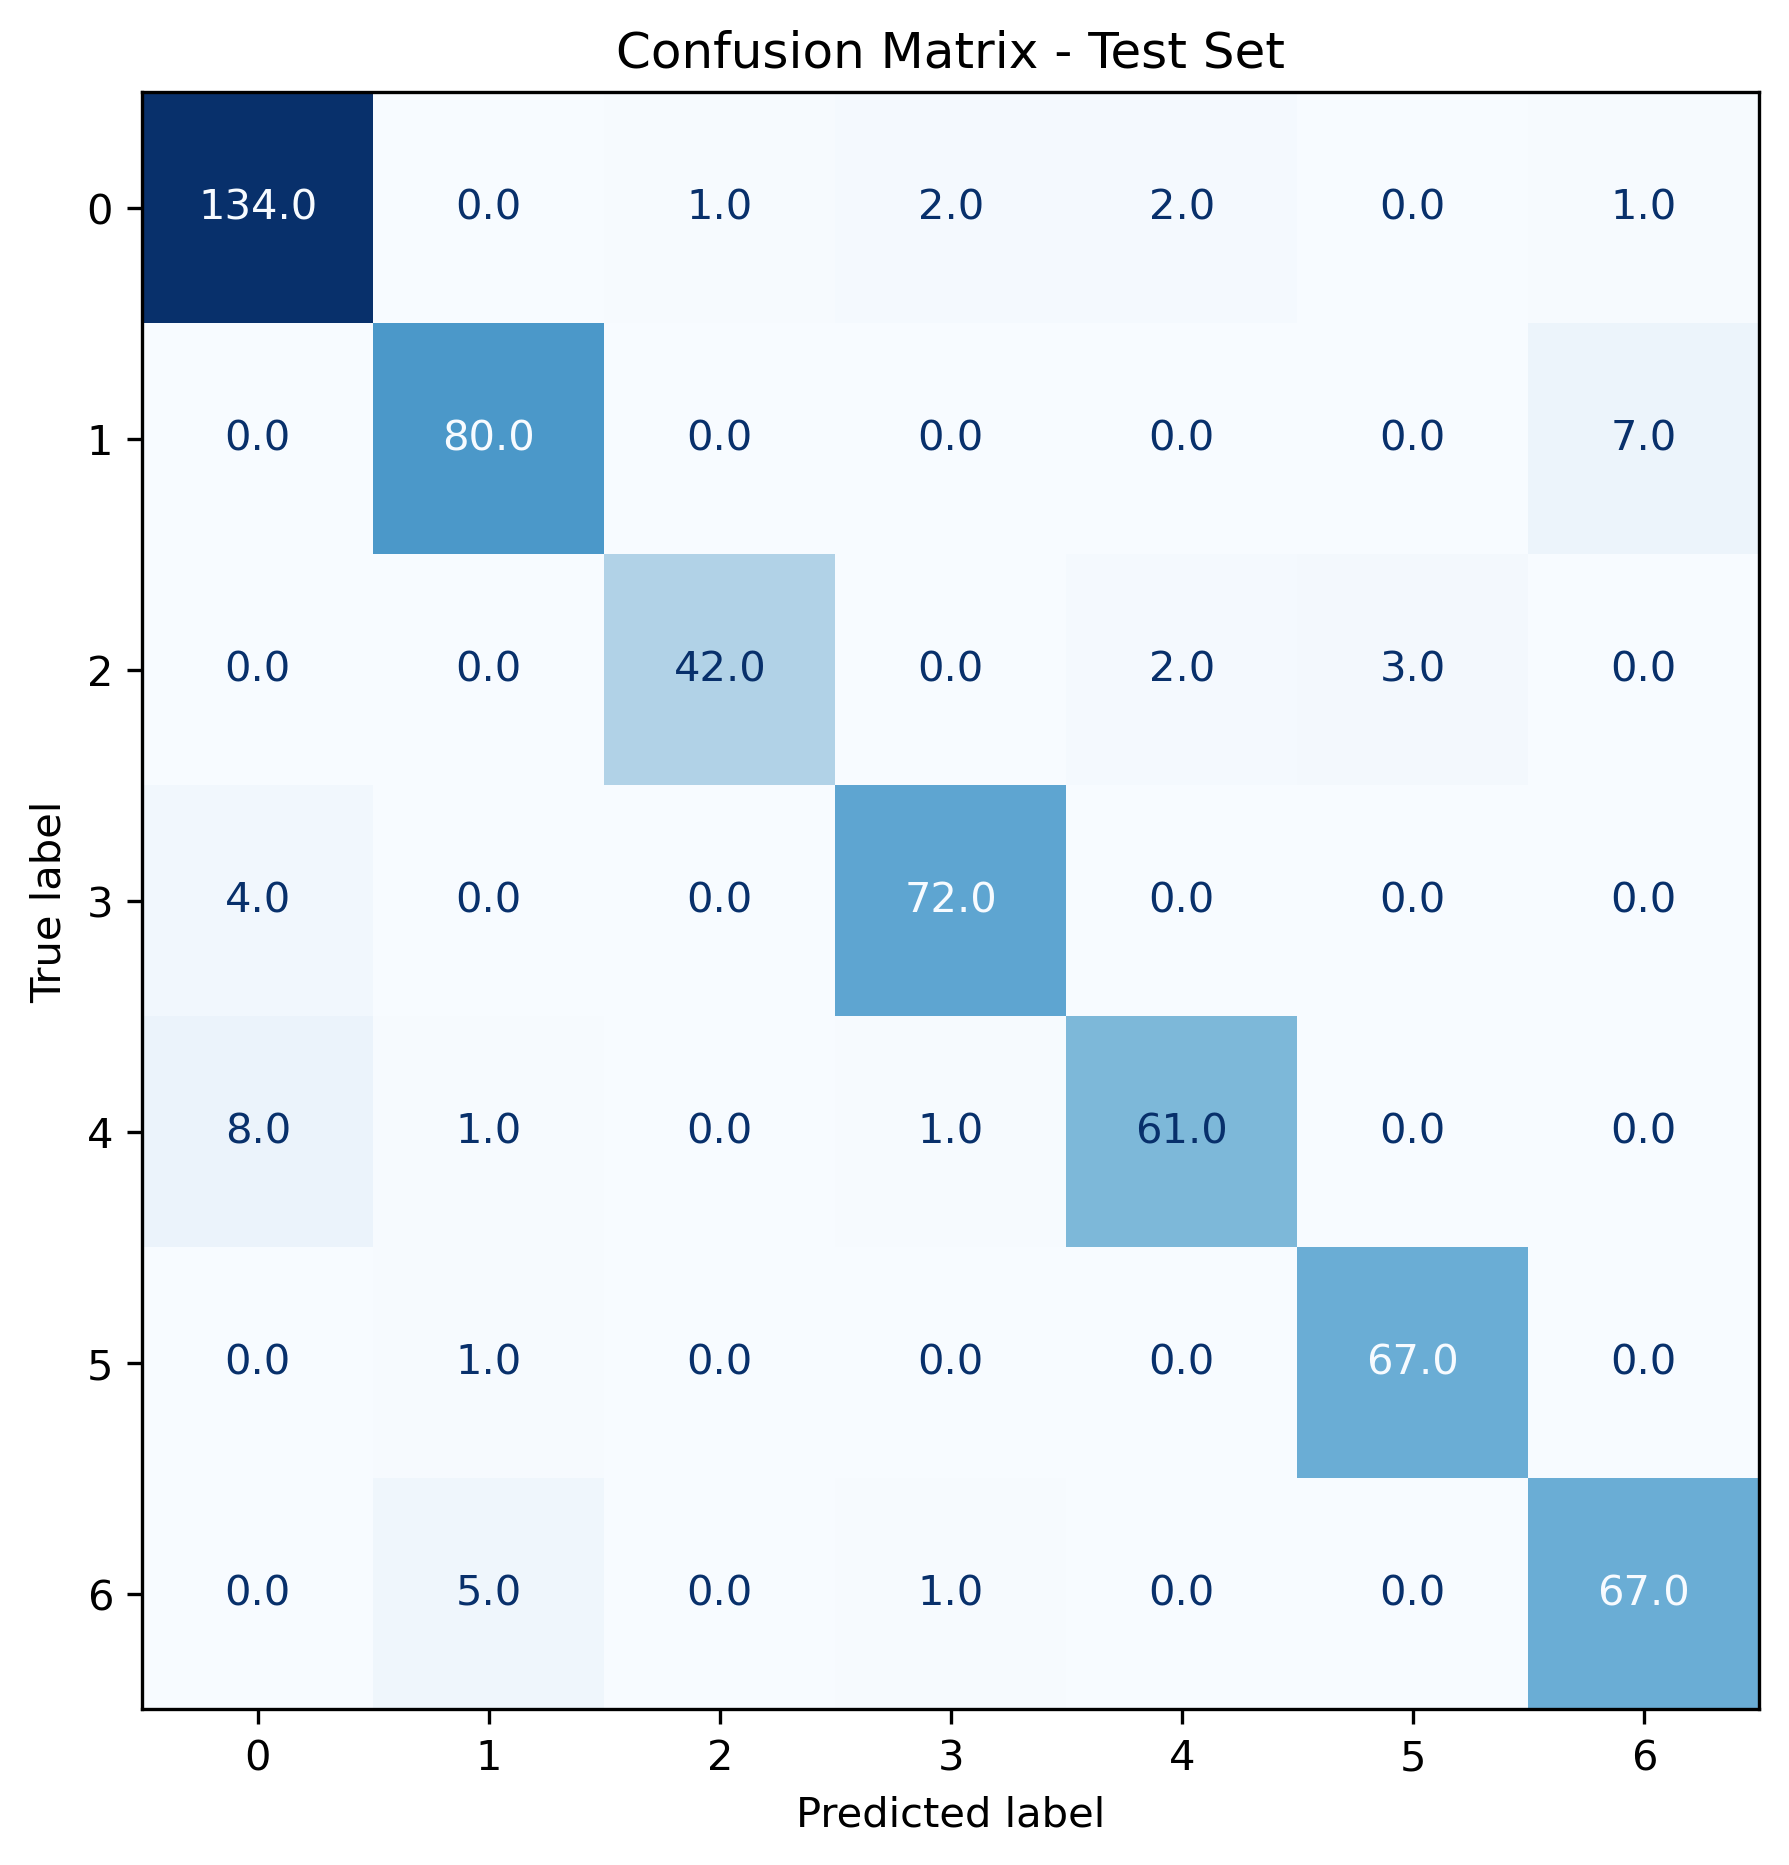
\includegraphics[width=0.7\linewidth]{../cnnlstm_loss1_cm.png}}
		\caption{ماتریس آشفتگی - مدل \lr{CNN-LSTM}}
		\label{fig:cnnlstm_cm} 
	\end{figure}\\
	\clearpage
	\section{تحلیل نتایج}
	با مقایسه دقت نهایی و نمودار دقت در روند تربیت برای داده‌های تربیت و اعتبارسنجی می‌توان دو مدل \lr{CNN} و \lr{CNN-LSTM} را با هم مقایسه کرد. ابتدا از دقت که در 
	\autoref{tab:accuracy_cnn}
	و 
	\autoref{tab:accuracy_cnnlstm}
	آمده است می‌توان دریافت که همانطور که انتظار می‌رفت شبکه 
	\lr{CNN-LSTM}
	به خاطر بررسی ترتیب داده‌ها که در داده‌هایی مانند صوت حائز اهمیت است بهتر عمل می‌کند. علاوه بر این موضوع، چنانچه به شکل‌
	\autoref{fig:cnn_loss1}
	و 
	\autoref{fig:cnnlstm_loss1}
	توجه کنیم، می‌توانیم متوجه شویم که در حین روند تربیت، نه تنها همگرایی سریع‌تر رخ داده،‌ بلکه دقت داده‌های اعتبارسنجی نزدیک‌تر به داده‌های آموزش است. این موضوع در کنار دقت بالاتر مدل به تعمیم‌پذیری بهتر مدل 
	\lr{CNN-LSTM}
	اشاره دارد.\\
	در کنار این‌ها، با بررسی ماتریس آشفتگی می‌توان دید که مدل دارای شبکه \lr{LSTM} توانسته در ۶ کلاس از کل ۷ کلاس مقدار بیشتری کلاس صحبح را پیش‌بینی‌ کند. همچنین می‌توان مشاهده کرد که این مدل برای برخی از کلاس‌ها که به جای هم تشخیص داده می‌شدند،‌ رفتار بهتری دارد.
\end{document} 